\documentclass[a4paper, article, english, oneside, unknownkeysallowed, 12pt]{memoir} 
\usepackage{preamble}


\usepackage[
  backend=biber,
  style=authoryear-ibid,
  maxcitenames=2,  % show up to 2 authors in citations
  mincitenames=1,  % use "et al." if more than 2
  maxbibnames=10,  % show up to 10 names in bibliography
  minbibnames=1,
    uniquelist=false   
]{biblatex}


\addbibresource{causal_effect_schools.bib}

\AtEveryBibitem{%
  \clearfield{urlyear}%
  \clearfield{urlmonth}%
  \clearfield{urlday}%
  \clearfield{urldate}%
}

% Name and Title
\title{ High school value-added beyond achievement: effects on higher education application behavior}
\author{ Bruno E. Aravena-Magüida}
\date{May 2026}

% Header (top) and footer (bottom)
\pagestyle{fancy}
\fancyhead[R]{\emph{May Draft}}
 \fancyhead[L]{BEAM} % keep section names
\fancyfoot[R]{}
\fancyfoot[L]{}


\begin{document}

% Prints title block from macros given above
\maketitle

% Prints a table of contents
\setcounter{tocdepth}{2}
\renewcommand\contentsname{}
%\tableofcontents* 
%\clearpage

\section{Introduction}

%Higher education good and choices relevant
Economics literature has spent a lot of time measuring the returns to accessing higher education. 
Choice of institution and especially of major have also been proven to be very relevant in terms of labor market outcomes \parencite{kirkeboen_field_2016}.



%Choices higher ed. bad
Despite the stakes of this decision being very high, we have many reasons to think that these choices are sub-optimal.
The literature has documented important diparities in application and enrollment rates across different groups of students, as well as a series of interventions tackling different frictions which have proven relevant and pervasive in the process of applying and enrolling to higher education. 
\parencite{chetty_diversifying_2025,hoxby_what_2015, dynarski_closing_2021, hastings_informed_2016}.

%Do people go to college enough ? 
%-However, we do not know much how these frictions look in "equilibrium". 

In a context where these frictions are pervasive, reducing them is highly valuable. 
High schools potentially play an important role in inducing or alleviating such frictions, suggesting a different way to think about their value-added on top of achievement metrics.
However, measuring such effects requires both exogenous variation in school assignment as well as being able to observe both applications and enrollment in higher education. 
Both of these requirements are hard to meet, which has limited the literature on this topic.


In this paper, I take advantage of the Chilean policy and data landscape to estimate value added of schools on higher educational choices, while also examining their impact on traditional achievement outcomes. 
The centralized school assignment system in Chile \textit{(SAE)}, which breaks ties through lotteries provides exogenous variation to study these effects at a national scale. Moreover, the centralized higher education application system allows me to observe both application and enrollment choices. 

I proceed in 2 steps in order to make my results easier to understand. 
I first compute observational value-added for each school for a given outcome. 
This is equivalent to estimating a school-fixed effect in a regression with rich student controls.
These estimated values play an important role in the second step. 

In my second step I estimate an IV regression on the same outcome using the observational value-added as the value of the school offered (instrument) and the school attended (endogenous variable). 
This design allows me to answer the question of whether gains in the observational value-added metric induced by the lottery offers imply causal effects.
In particular, I can summarize my answers in a single number per outcome which will be reported across specifications. 
$\theta$ represents the 'pass-through' of the observational value-added metric to causal effects. 
If $\theta$ is close to one, that would indicate that gains in the value-added metric perfectly predict lottery-induced effects in that outcome. 
My estimates suggest that $\theta$ is between 0.835-0.841 for achievement tests and 0.674 for STEM enrollment. 
In practical terms this allows me to answer how informative would the observational value-added metric be for a family that is trying to choose a school for their child, if they were to use it as a guide, in a similar spirit to \textcite{angrist_leveraging_2017}.


%(these effects are meaningless without a sense of variance of the metric)

%(orthogonal VA?)

%### Small Conclusion (check content)

The results in this paper suggest that schools play an important role not only in higher educational choices not only through academic achievement, but also with measureable effects on important elements such as institutional quality or major choice. 
I take this to be the first paper that paints such a detailed picture of the effects of the high school system on higher education. 
All in all, these results invite families, researchers, and policy-makers to think about the school value-added in a far more comprehensive way than it has been previously discussed by the literature.


This paper connects many strands of literatures. 
Firstly, I hope to extend existing work on the value-added of schools and teachers \parencite{chetty_measuring_2014},  

\parencite{dobbie_medium-term_2015, beuermann_what_2023}




College Application frictions and interventions. 
\parencite{chetty_diversifying_2025,hoxby_what_2015, dynarski_closing_2021, hastings_informed_2016}.


 In line with these arguments,  \parencite{abdulkadiroglu_elite_2014} and 
\parencite{abdulkadiroglu_parents_2020} are some of the only papers to report causal effect of schools on some measure of quality of college enrolled. Yet, these papers are unable to assess whether these effects operate through increases in application rates, acceptance rates or enrollment rate. Moreover, they do not speak to how schools might affect major choice. 

Causal effects of schools using lotteries and/or centralized assignment. 
\parencite{abdulkadiroglu_research_2017}
\parencite{abdulkadiroglu_elite_2014}


The rest of the paper is organized as follows.
Section 2 describes the context and data.  (easy)
Section 3 describes the methodology employed.  (mid)
Section 4 presents the results. (mid)
Section 5 concludes. (easy)






Assessing a school's quality has been an important concern for families, governments and researchers. 
For the most part, the economics literature has focused for in outcomes such as achievement scores in  standardized tests and college exams, considering them as proxies for later relevant variables such as college or labor market outcomes. \parencite{chetty_measuring_2014}\footnote{ More recently, the literature has also measured other socially-relevant outcomes such as teenage pregnancy, incarceration and substance use \parencite{dobbie_medium-term_2015, beuermann_what_2023}.}. 

Many of the attempts to measure direct effects on higher education have been limited to a crude set of outcomes such as college enrollment or number of academic semesters \parencite{angrist_stand_2016, dobbie_medium-term_2015}\footnote{An important exception on this regard is \parencite{dobbie_charter_2020} where the authors can directly observe labor market outcomes, but giving up exogenous variation in their study.}.


I argue that this is an insufficient way to characterize the effects of schools on later outcomes: There are important differences across institutions and programs that make the time spent at a higher education institution too coarse.
I discuss on this paper the role of selectivity/quality of the higher education institution, as well as the choice of field of occupation. Intuitively: a school with that places their students in more selective institutions or higher pay programs will have alumni should be considered to have a different causal effect than another one -with a similar incoming student pool- that places their students in less selective institutions or lower pay programs, even if they have similar college enrollment and retention rates. 
 In line with these arguments,  \parencite{abdulkadiroglu_elite_2014} and 
\parencite{abdulkadiroglu_parents_2020} are some of the only papers to report causal effect of schools on some measure of quality of college enrolled. Yet, these papers are unable to assess whether these effects operate through increases in application rates, acceptance rates or enrollment rate. Moreover, they do not speak to how schools might affect major choice. 

Evidently these effects could entirely be driven by achievement effects. 
However, there is evidence to think that there are important margins on the college choice decision that are not determined by scores.  
For instance, the fact that lower-income students are less likely to apply to selective institutions than their higher-income peers of the same achievement level has been documented multiple times  \parencite{dynarski_closing_2021} \parencite{chetty_diversifying_2025}, and simple interventions  \parencite{hoxby_what_2015} have proven successful in closing this gap.
 If schools differ on the type of institutions they might induce their students to apply to, there might be important effects that the metrics such as college enrollment or number of semesters would fail to capture. 


Another example is how information about returns might change major choice.
 We know that the returns to higher education education vary enormously across fields \parencite{kirkeboen_field_2016} and that interventions such as information provision -which do not change achievement- can help move students move towards higher return programs \parencite{hastings_informed_2016}. 

To the extent that different schools provide more accurate information about the returns to college and fields, they might nudge students int higher education and into high-pay majors.
 However, incomplete or wrong information might push into other fields. Other than education, schools might also affect this choice through other channels such as non-tested cognitive skills, non-cognitive skills or preferences.  
 In this paper I attempt to show that schools induce differences on higher education choices through both achievement and non-achievement channels.









\clearpage
\section{Context and Data}

\subsection{Institutional Setting}

Chile is a useful setting for this project because both school enrollment and higher-education choices are recorded in national administrative data. Formal secondary education begins in grade 9 and lasts four years. Students may attend public, private-subsidized, or private non-subsidized schools. Public and private-subsidized schools are publicly financed and participate in the centralized school assignment system described below; private non-subsidized schools remain outside that assignment mechanism. This distinction is useful for estimation: the administrative panel follows students across the full school system, while the lottery variation comes from students applying to participating schools.

I define the main school exposure using the school identifier (RBD) where a student spends the most time after grade 8. This definition smooths over short enrollment spells and transfers, and it gives a single high-school measure for each student. The cleaned panel also tracks annual enrollment, attendance, and grades, which allows me to construct pre-treatment middle-school controls such as the school most attended in grades 5 to 8 and standardized measures of grades and attendance before high school.

\subsection{Student Panel and Baseline Controls}

The broad analysis panel starts from the universe of students first observed in grade 8 between 2017 and 2020. This produces 944,360 students across four cohorts. The panel contains 238,467 students in the 2017 grade-8 cohort, 232,498 in 2018, 233,401 in 2019, and 239,994 in 2020. Students can be followed over time with a scrambled individual identifier, and the main high-school exposure is observed for 4,133 RBDs.

Baseline achievement comes from SIMCE, Chile's national standardized assessment system. SIMCE is administered in different grades depending on the year, including grades 4, 8, and 10. Because the COVID-19 pandemic disrupted testing in 2020 and 2021, grade-8 and grade-10 measures are not available for all cohorts in the same way. I therefore use grade-4 SIMCE as the main pre-treatment achievement control. This gives a nationally comparable measure of math and language skills before high-school assignment for 771,968 students in the broad panel.

The SIMCE files also contain parent-survey information. I use these surveys to measure family background before treatment, including household income, parental education, indigenous origin of the parents, and early-childhood attendance. These variables are useful because they proxy for family resources and prior investments that may influence both high-school choices and later higher-education outcomes. When parent-survey variables are missing, I use pre-treatment school and neighborhood cells to impute medians where enough donor observations are available; remaining missing values are left missing.

\begin{table}[H]
\centering
\caption{Main data sources and sample sizes}
\label{tab:data-samples}
\begin{tabular}{lr}
\toprule
Sample or outcome availability & Students \\
\midrule
Broad grade-8 universe, 2017--2020 & 944,360 \\
With grade-4 SIMCE math and language controls & 771,968 \\
With valid higher-education math admission-test outcome & 640,078 \\
\midrule
SAE lottery sample with assignment risk & 163,600 \\
SAE lottery sample with math outcome & 103,941 \\
\bottomrule
\end{tabular}
\end{table}

\subsection{Centralized School Assignment}

Chile's centralized school assignment system, the Sistema de Admision Escolar (SAE), assigns students to participating schools through a version of student-proposing Deferred Acceptance. Families submit ranked lists of schools. The mechanism combines these rankings with school vacancies and priority rules, and it uses random tie-breakers when there are more applicants than seats within a priority group. Conditional on the information that determines assignment probabilities, these tie-breakers generate the quasi-experimental variation used in the empirical design.

I use applications to grade-9 vacancies to construct the lottery sample. The estimation sample consists of timely SAE applicants with assignment risk, meaning that no single school is assigned with probability one in the simulated assignment data. This sample contains 163,600 students from the 2018--2020 cohorts. On average, these students have positive simulated assignment probability at about 3.1 schools; the median is 3 and the 90th percentile is 5. About 86.5\% receive a nonzero first-round offer. The first-round offered RBD is the source of the instrument, while the student's realized high-school exposure is measured by the most-time RBD described above.

The value-added exercise uses the broader student panel, while the causal estimates use the smaller lottery-risk sample. This distinction is important. The broad panel improves precision in estimating school-level outcome gradients. The lottery sample then asks whether lottery-induced movement toward schools with higher measured value added causes improvements in the same outcomes.

\subsection{Higher-Education Outcomes}

The higher-education system also generates administrative data at the student-program level. Students applying to selective higher education take a national entrance exam: the PSU through 2020, the PTU in 2021--2022, and the PAES from 2023 onward. The mandatory components measure math and verbal skills. Students may also take optional exams in history and social sciences, natural sciences, and advanced mathematics. I use the mandatory math and language scores as achievement outcomes, standardizing them within test year to make them comparable across test regimes.

Higher-education applications and admissions are organized at the program-institution level. A student's admission depends on entrance-exam scores, school GPA-based scores, ranked program preferences, and the weights each program assigns to score components. This structure is useful because it makes higher-education choices much richer than a single college-enrollment indicator: students choose not only whether to enroll, but also which institution, program, and field to pursue.

I link the school panel to higher-education matricula records for first observed enrollment. The main non-achievement outcome is an indicator for enrollment in a STEM program, defined from the field classification of the first higher-education enrollment. I also construct measures of program and institution accreditation. In particular, program-certified years multiply an indicator for whether the program is accredited by the number of years for which the institution is accredited. These outcomes allow me to study whether high schools affect the type and quality of higher-education option students enter, not just whether students enter higher education at all.

Students without an observed higher-education enrollment are coded as zero for unconditional enrollment outcomes such as STEM enrollment. For accreditation-years outcomes, non-enrollment is also coded as zero, while observed enrollment records with missing accreditation inputs are left missing. In the broad panel, 626,413 students have a first higher-education enrollment record, and the unconditional STEM enrollment rate is 20.9\%.

\subsection{School Value-Added Measures}

For each outcome, I construct observational school value added using the broad student panel. The adjusted value-added measure is the school fixed effect from a student-level regression with cohort, demographic, baseline SIMCE, family-background, and middle-school controls. The All-sample value-added file contains 4,068 schools and 42 outcome transformations. Controlled math value added is available for 3,365 schools, controlled language value added for 3,374 schools, and controlled STEM and accreditation value added for 3,685 schools.

These school measures are not interpreted as causal by themselves. They summarize how students linked to a school perform after adjusting for rich pre-treatment information. The causal analysis uses the SAE lotteries to ask whether being offered and then attending schools with higher observational value added improves student outcomes.



\clearpage 
\section{Empirical Framework}



This document presents an update on the progress of my research project. I begin by outlining the conceptual framework and identification strategy guiding the analysis.

The project focuses on estimating the effect of schools on students’ choice of major in higher education, with particular attention to whether these effects operate through academic achievement (test scores) or through non-score mechanisms.

I then introduce the reduced-form specifications used to estimate school effects on the main outcomes, along with a strategy to provide evidence on non-score channels in major choice.
In addition, I discuss a structural model of major choice that may help disentangle these mechanisms. Finally, I describe progress in replicating school assignments in the Chilean centralized system and outline procedures to compute assignment probabilities.


In this section I describe how I am currently thinking of my analysis. I review the assumptions and methodologies related to the estimation of school specific effects using centralized assignment mechanisms, and then I present the main reduced-form regressions I intend to run, as well as some challenges and how I intend to address them.

\subsection{Potential Outcomes and School Effects}

For this section I borrow from \textcite{angrist_credible_2024} and \textcite{abdulkadiroglu_research_2017}

Suppose $N$ students and $J$ schools. 
Following the value-added literature on school effectiveness,  I assume a constant-effects model. Then, the potential outcome $Y_{ij}$ of a student $i$ in a school $j$ is additively separable and can be written as: 
\begin{equation}
  Y_{ij} = \nu_j + \epsilon_i
  \label{linear-separable}
\end{equation}

Hence, the causal effect of attending a school $j$ relative to $k$ would be given by $\nu_j - \nu_k$.


By adding a constant, we can renormalize this model relative to the average achievement ($\beta_0 = \frac{1}{J}\sum_{j=1}^J \nu_j$ )
As a result, we can rewrite the model as: 

\begin{equation}
 Y_i = \beta_0 + \sum_{j=1}^J \beta_j D_{ij} + \epsilon_i 
  \label{base}
\end{equation}

where now $\beta_j = \nu_j - \beta_0$. 

Unless school assignment is completely random, the evident threat to running this regression is the fact that $\cov(\epsilon_i, D_{ij})$ might be different than zero. 
This selection bias would bias our estimates and prevent a causal interpretation.


\subsubsection{Assignment Mechanisms and Assignment Risk}
A common strategy used in research to overcome this issue is the use of individual school lotteries, and more recently, centralized school assignments. 
In centralized assignment mechanisms, applicants submit rank-ordered preferences over schools ($\succ_i$) at which they might also have different priority levels\footnote{e.g. in the Chilean case being the child of a member of the school staff gives a student priority in that school.}.
These priorities operate as the school's preferences for students. An algorithm in place (most commonly student-proposing Deferred Acceptance) takes these preferences and outputs a school assignment ($Z_{ij}$) with one offer per student.
In order to break ties of students with the same preference and priority level, these systems randomize. 

If we refer to a student's priority at each school as $\rho_i = (\rho_{i1}, ...,\rho_{iJ})'$, we can define a student's type as the combination of both $\theta_i \equiv (\succ_i, \rho_i)$.
Let the probabilities of admission at a school be given by $p_i = (p_{i1}, ..., p_{ij})'$, with $p_{ij} = Pr(Z_{ij} = 1)$.

The mechanism described above implies that students with the same preferences and priority vector have the same probability of being assigned to the schools in their portfolio, which is called by \textcite{abdulkadiroglu_research_2017} the `equal treatment of equals' (ETE) property. 
Formally ETE states $\theta_i = \theta_j \implies p_i = p_j$. 

They also prove that under ETE that for any observed characteristic fixed under re-randomization $W_i$ (i.e. pre-assignment or not affected by assignment) we have that:
\begin{equation}
 Pr[Z_{ij} = 1|\, W_i = w, \theta_i = \theta] = Pr[Z_{ij} = 1 | \, \theta_i = \theta]  
\end{equation}

Hence, for any such variable $W_i$ we can write 
\begin{equation}
 W_i \ind Z_i \, | \, \theta_i 
 \label{w ind}  
\end{equation}

In particular, and as a consequence of equation \ref{linear-separable}, where we assumed ability $\epsilon_i$ to be fixed under re-randomization, partly due to the absence of match effects, we can write
\begin{equation}
  \epsilon_i \ind Z_i \, | \, \theta_i   
\end{equation}

This is the key identifying assumption of the design.
It states that conditional on the student type, the school offer is exogenous to the error term (in this example student's ability).
Under this assumption and perfect compliance ($Z_i = D_i$), we could estimate equation \ref{base} by saturating on an indicator for each student type $\theta_i$. 

However, that is often not feasible as these strata are too granular to have enough variation within each of them to estimate the model. 
As described by \textcite{angrist_credible_2024}: "In practice (...) we see nearly as many preference and priority combinations as there are students in a match."  
A solution to this issue is to use the probabilities of admissions as propensity scores to pool over student types, as proposed by \textcite{abdulkadiroglu_research_2017}. 
This is an application of the propensity score methods \parencite{rosenbaum_central_1983} and it yields:  
\begin{equation}
  \epsilon_i \ind Z_i \, | \, p_i 
  \label{CRA}
\end{equation}

Note that by eq. \ref{w ind} we can also consider other control variables (as long as they are fixed under re-randomization). Thus for any pre-treatment covariate $X_i$ it must be the case that 
($\epsilon_i, X_i) \ind Z_i | \theta_i$, so we can rewrite Eq \ref{CRA} as $  \epsilon_i \ind Z_i \, | \, (p_i, X_i) $ to allow for such controls.

\subsubsection{Towards Conditional Independence Assignment}

Although an instrumental variables approach may seem natural given the availability of many exogenous instruments, estimation of school-specific effects suggests otherwise. The issue arises from the multiplicity of (unordered) outside options. 
Individuals instrumented into a school may come from different margins, and as a result interpretation becomes challenging unless strong assumptions are made \parencite{angrist_methods_2023} \parencite{kirkeboen_field_2016}.  
To see this, consider students with an identical ranked list of three schools who are guaranteed admission to their third choice if they are not successful in their first two applications. An offer to the first school then generates two margins of compliance.
The problem becomes more complex when students have different fallback options or when identical preference lists are rare in the data.

Instead, to compute effects at the school level, the literature typically relies on selection on observables i.e. the construction of a control vector $X_i$ such that $ \epsilon_i \ind D_i \, | \, (X_i)$.
Note that under the constant effects assumption and the ETE property of lotteries, equation \ref{CRA} is closely related to this framework. 

An additional assumption that allows us to move from equation \ref{CRA} to a conditional independence framework is that compliance with offers is as good as random.
The argument for this assumption is that all sorting occurs at the application stage, and thus captured by the individual type $\theta_i$, and that post-offer compliance is determined by idiosyncratic shocks uncorrelated with the error term (in this case ability $\epsilon_i$).
This argument is often credited to \textcite{dale_estimating_2002}. 

\begin{equation}
  \epsilon_i \ind D_i  \mid (p_i) 
  \label{CIA}
\end{equation}

Compliance being as good as random yields a traditional conditional independence assumption, from where estimation is straightforward. 
%Note that we can add controls to the conditioning set 
%In particular, if covariates used are lagged (pre-treatment) outcomes we end up with a Risk Controlled Value Added Model (RC VAM) as constructed in (centralized VAM paper). 

%\begin{equation}
%  Y_i = \alpha_0 + \sum_j \alpha_j D_{ij} + X_i' \Gamma + g(p_i) + \eta_i 
%\end{equation}

\subsection{Estimation in specific outcomes}

In this subsection I present the main regressions I intend to run, as well as an approach to provide reduced-form evidence for a non-score mechanism of schools on major choice.
Let $Y^{MATH}_i$ represent the outcome of a student in the standardized exam for mathematics and $Y^{STEM}_i$ an indicator variable for whether the student enrolls in a STEM program. 

Let $X_i$ be a vector of characteristics not changed by treatment (e.g. demographics), and $Y^{MATH}_{pre,i}$ a measure of pre-treatment math achievement .

Following equation \ref{CIA} I write:

\begin{equation}
  Y^{MATH}_i = b_0 + \sum_j b_j D_{ij} +  X_i' B + b_{pre} Y^{MATH}_{pre,i} +   g(p_i) + \epsilon_i 
  \label{Math}
\end{equation}


\begin{equation}
  Y^{STEM}_i = c_0 + \sum_j c_j D_{ij} + X_i' C + g(p_i) + \eta_i 
  \label{STEM_prev}
\end{equation}

The only difference between these two regressions is the fact that I propose to include a lagged outcome (pre-treatment math achievement) on the first regression.
I do not have a similar lagged outcome for STEM enrollment. 
The inclusion of lagged outcome for math achievement makes \ref{Math} an `RC VAM' regression under the \textcite{angrist_credible_2024} terminology. While \ref{STEM_prev} is a Risk-Controlled OLS or what \textcite{angrist_credible_2024} calls `Risk only'. 

Remember that, under the CIA assumption above, these regressions could be run without any of the controls and should still hold causal interpretation: the CIA assumption only needs the $p_i$ to be included.



\clearpage 
\section{Results}

I organize the results in three blocks. First, I report the main pass-through
estimates for four scalar value-added measures: two achievement measures and two
higher-education measures. Second, I ask whether these pass-through estimates
vary by baseline achievement, using grade-4 math achievement quartiles. Third, I
use the two-dimensional value-added construction to separate math value added
from the component of STEM value added that is orthogonal to math value added.

\subsection{Main Value-Added Estimates}

Table~\ref{tab:main-four-va-results} reports the main IV estimates. Each column
uses the same outcome to construct the observational school value-added measure,
the lottery-induced expected value-added instrument, and the realized attended
school value-added treatment. The coefficients can therefore be read as
pass-through estimates: how much a lottery-induced increase in a school's
observational value added translates into a causal gain in the corresponding
student outcome.

The achievement estimates are close to one. A one standard deviation increase in
school math value added raises math achievement by 0.841 standard deviations,
while the analogous estimate for language is 0.835. The higher-education
estimates are also positive, though somewhat smaller and less precise. The
estimated pass-through is 0.674 for STEM enrollment and 0.788 for the
program-certified-years outcome. Taken together, the estimates suggest that the
observational school value-added measures are informative not only about test
score production, but also about later higher-education choices.

\begin{table}[!htbp]
\centering
\caption{Main scalar school-value IV estimates}
\label{tab:main-four-va-results}
\begin{tabular}{lcccc}
\toprule
 & \multicolumn{2}{c}{Achievement} & \multicolumn{2}{c}{Higher education} \\
\cmidrule(lr){2-3} \cmidrule(lr){4-5}
 & Math & Language & STEM enrollment & Institution quality \\
\midrule
$\theta$ & 0.841 & 0.835 & 0.674 & 0.680 \\
SE & (0.071) & (0.082) & (0.065) & (0.095) \\
Observations & 90,906 & 92,472 & 135,898 & 135,898 \\
\bottomrule
\end{tabular}
\end{table}


\subsection{Heterogeneity by Baseline Achievement}

Figure~\ref{fig:simce4-math-quartile-four-metrics} repeats the same four
estimates separately by quartiles of baseline grade-4 math achievement. This
comparison is useful because it keeps the heterogeneity split pre-treatment and
available for the full analysis sample.

The achievement pass-through estimates increase with baseline math achievement,
especially for math value added. In the bottom quartile, the math estimate is
small and imprecise, while in the top quartile it is above one. The language
estimates follow a similar, though less monotone, pattern. In contrast, the STEM
enrollment estimates are stable across the baseline achievement distribution,
with point estimates between 0.64 and 0.73 in all four quartiles. The
program-certified-years estimates are noisier, but remain positive in the upper
three quartiles. This pattern suggests that the test-score value-added measures
may be more predictive for higher-achieving baseline students, while the
higher-education value-added measure for STEM enrollment appears to travel more
evenly across baseline achievement groups.

\begin{figure}[!htbp]
\centering
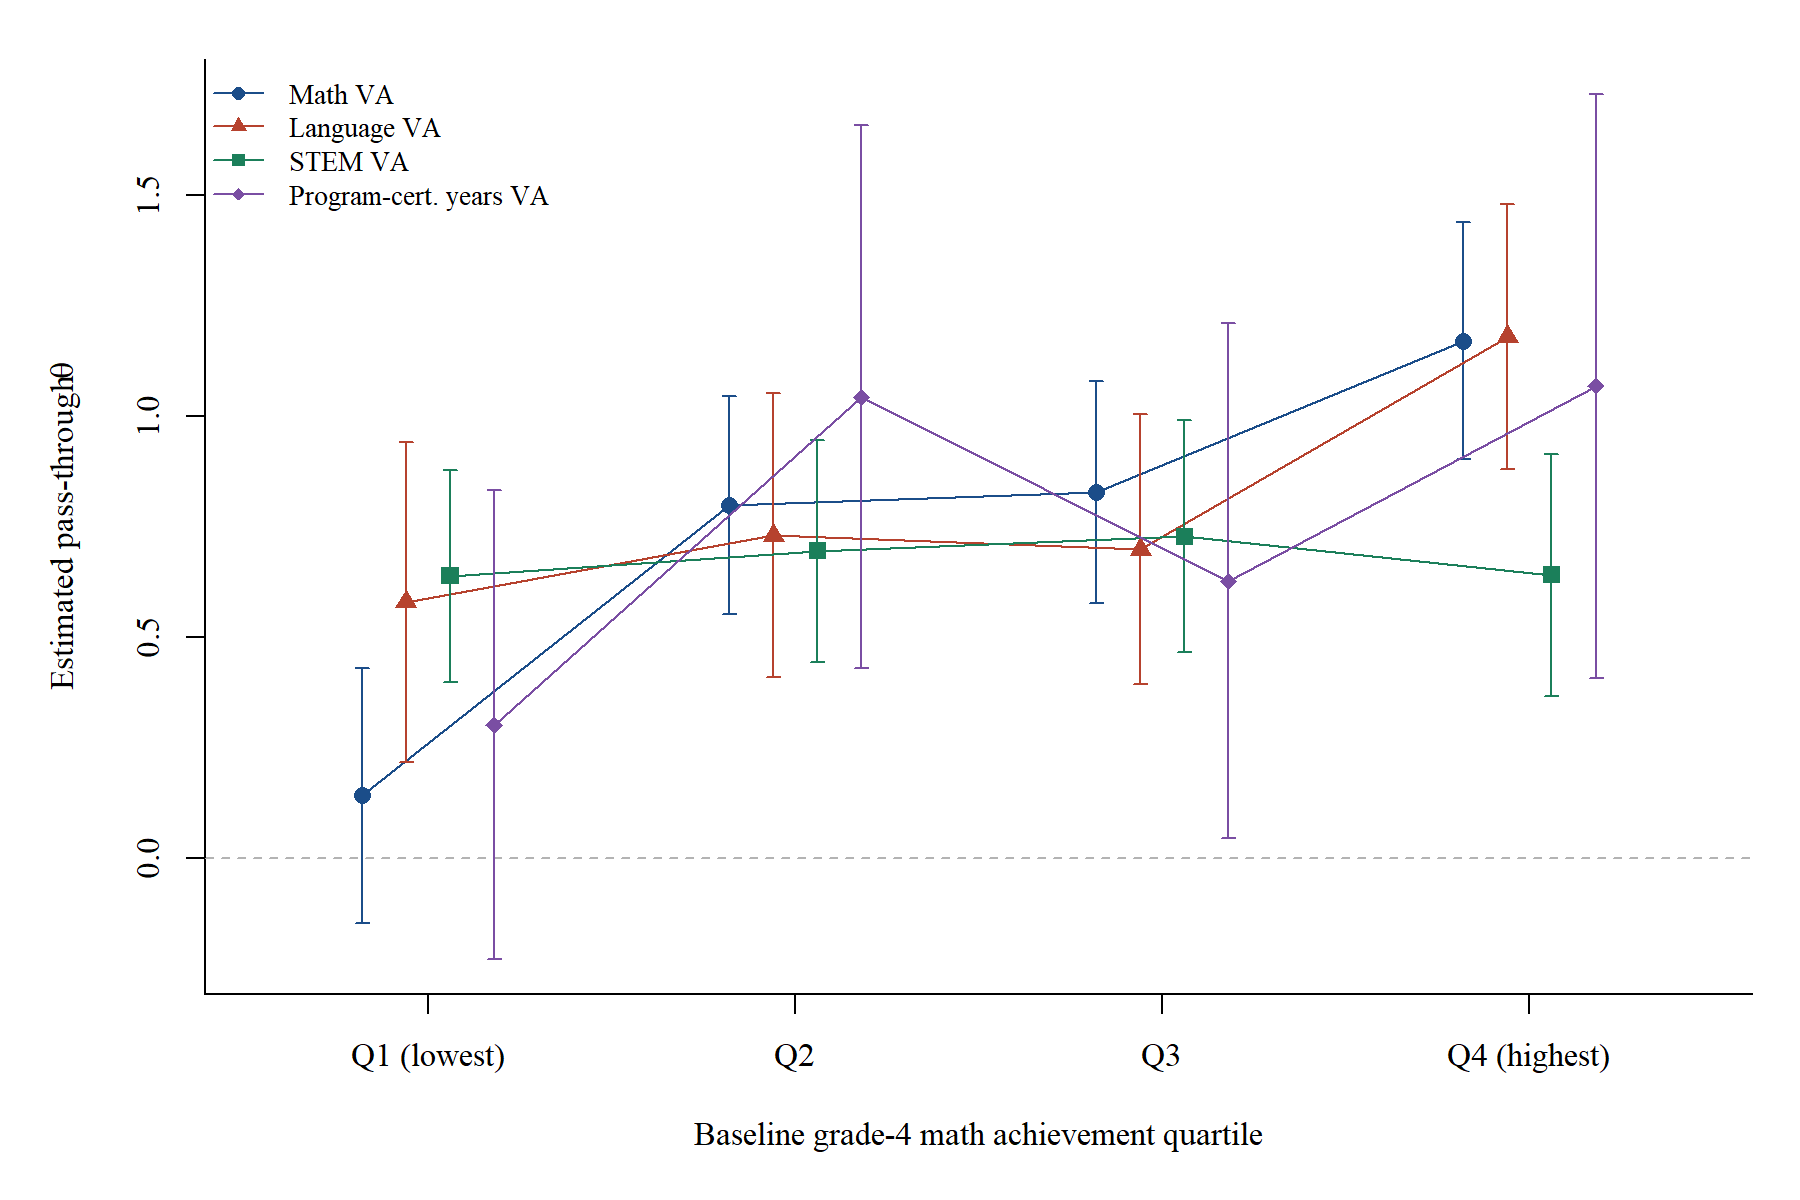
\includegraphics[width=.9\textwidth]{../../output/figures/results_section/simce4_math_quartile_four_metrics.png}
\caption{Scalar school-value IV estimates by baseline grade-4 math achievement quartile}
\label{fig:simce4-math-quartile-four-metrics}
\end{figure}
\FloatBarrier

\subsection{Orthogonal Math and STEM Value Added}

The scalar estimates above treat each outcome-specific value-added measure one at
a time. I also construct a two-dimensional measure that separates math value
added from STEM-enrollment value added. Figure~\ref{fig:math-stem-va-correlation}
shows that the raw school-level relationship between math value added and STEM
enrollment value added is positive but weak. This makes it possible to ask
whether schools that improve STEM enrollment are doing so only because they are
also high math value-added schools, or whether there is a distinct STEM-related
component.

\begin{figure}[!htbp]
\centering
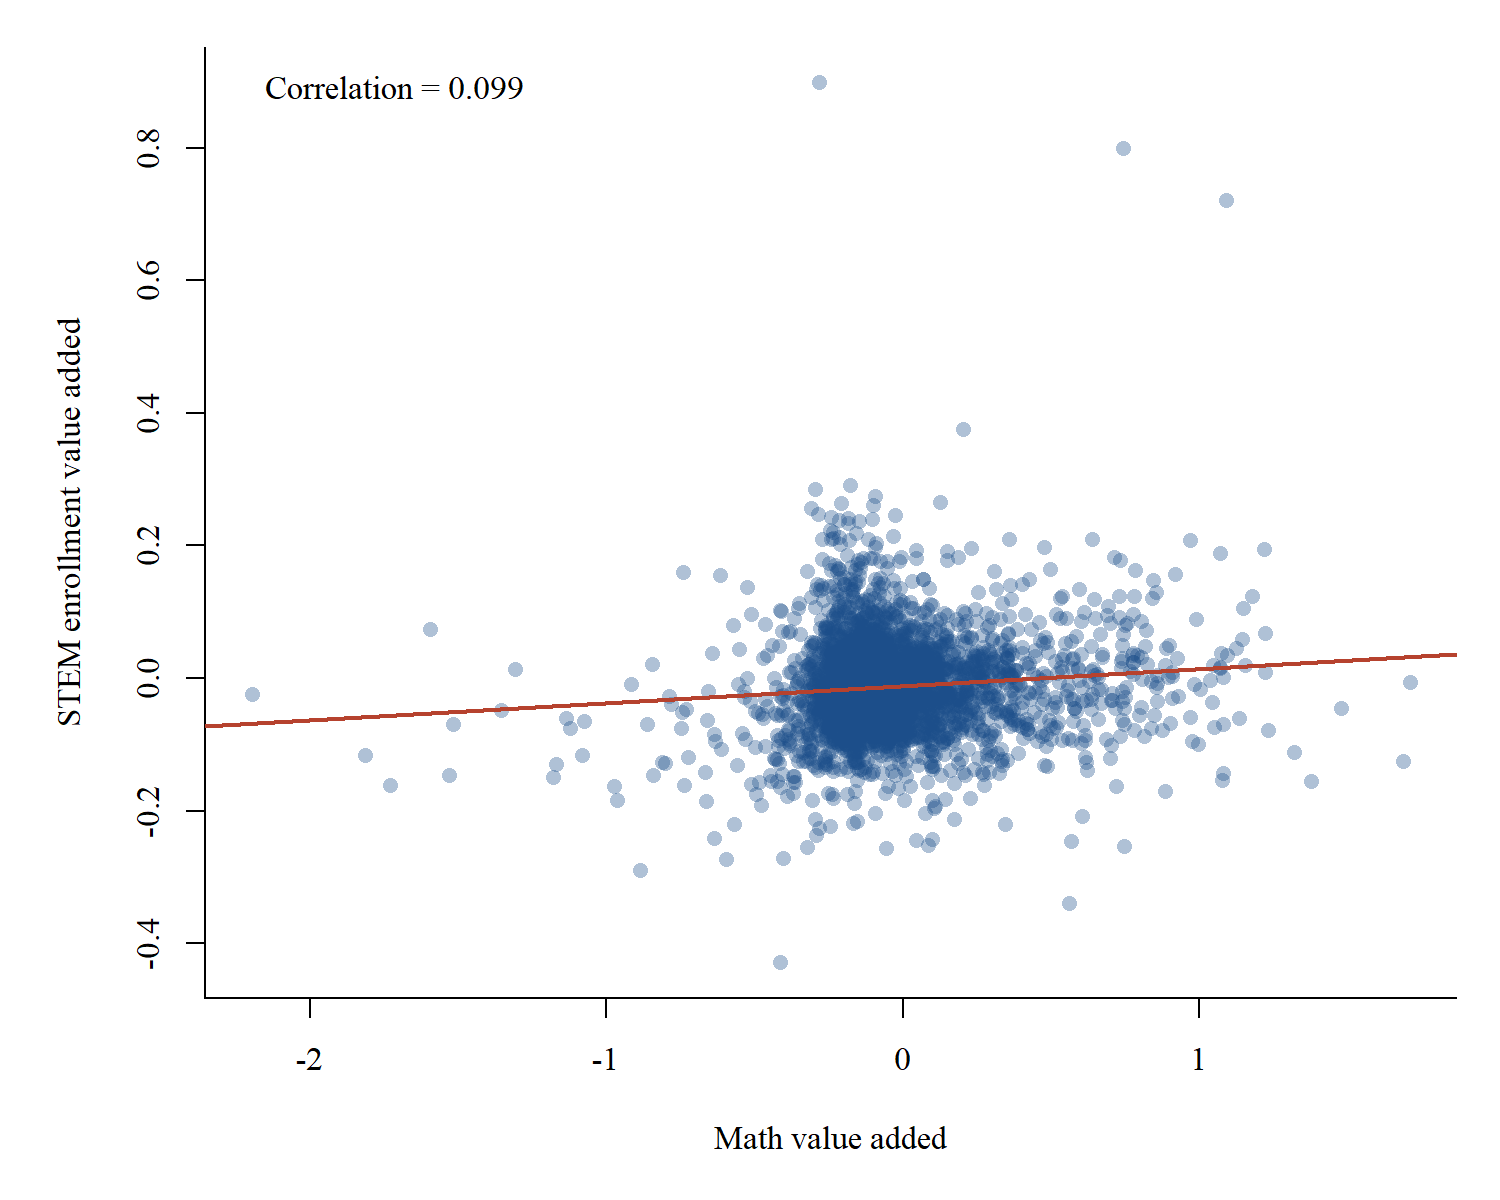
\includegraphics[width=.72\textwidth]{../../output/figures/results_section/math_stem_va_correlation.png}
\caption{Relationship between math and STEM observational value added}
\label{fig:math-stem-va-correlation}
\end{figure}
\FloatBarrier

Table~\ref{tab:orthogonal_school_va_iv_2x2} reports the corresponding
two-regressor IV estimates. Math value added strongly predicts math achievement,
with an estimate of 0.844, but it does not predict STEM enrollment once the
orthogonal STEM component is included. Conversely, the STEM component
orthogonalized against math value added strongly predicts STEM enrollment, with
an estimate of 0.656, while it has essentially no relationship with math
achievement. This supports the interpretation that schools differ along at least
two dimensions: one dimension that raises measured achievement, and another that
raises STEM enrollment conditional on achievement value added.

\begin{table}[!htbp]
\centering
\caption{Two-dimensional orthogonal school-value IV estimates}
\label{tab:orthogonal_school_va_iv_2x2}
\begin{tabular}{lcc}
\toprule
 & Math score & STEM enrollment \\
\midrule
Math VA & 0.844 & -0.058 \\
 & (0.072) & (0.039) \\
STEM VA orthogonal to math & 0.017 & 0.656 \\
 & (0.111) & (0.066) \\
\bottomrule
\end{tabular}
\end{table}


\FloatBarrier

\clearpage 
\section{Conclusion}


\clearpage
\printbibliography
\end{document}





















\end{document}
